\chapter{Range-Rename}
\label{chap:rename}

This chapter discribes the \bet operation, range-rename, that makes efficient
renames possible on full-path-indexed \betrfs.
To perform a rename, \betrfs simply calls the range-rename function of \fti,
which updates all related key/value pairs in the underlying \bets efficiently.
This chapter starts by describing the range-rename interface,
then explains how the range-rename operation updates large amounts of key/value
pairs efficiently through two techniques, tree surgery and key lifting.

\section{The range-rename interface}

Range-rename is a new key/value store function defined as:
range-rename(\spre, \dpre).
Generally speaking, range-rename(\spre, \dpre) does three things:
\begin{itemize}
\item it deletes all key/value pairs whose key has prefix \dpre from the
key/value store;
\item then, for any key/value pair $(k,v)$ in the key/value store whose key $k$
is the concatenation of \spre and a certain suffix $s$, it inserts a key/value
pair $(k',v)$ to the key/value store whose key $k'$ is the concatenation of
\dpre and the same suffix $s$;
\item at last, it deletes all key/value pairs whose key has prefix \spre in the
key/value store.
\end{itemize}

To see how range-rename accomplishes renames in full-path-indexed \betrfs,
consider renaming file ``/foo'' to ``/bar''.
In \mdb, \betrfs needs to insert the destination key ``/bar'' and deletes the
source key ``/bar'', resulting in two function calls to \fti.
On the other hand, in \ddb, \betrfs needs to delete all data keys of ``/bar''
(POSIX allows file renames to overwrite the destination file) and mutates all
data keys of ``/foo'' to be data keys of ``/bar'', which is the same as
range-rename(``/foo'',``/bar'') (data keys are the concatenation of the
full-path and an 8-byte block number).

Similarly, consider renaming directory ``/baz'' to ``/qux''.
In \mdb, \betrfs also needs to insert the destination key ``/qux'' and deletes
the source key ``/baz'' with two functions calls to \fti.
Additionally, \betrfs needs to mutates all keys with prefix ``/baz/'' to have
prefix ``/qux/'', which is covered in range-rename(``/baz/'', ``/qux/'')
(POSIX only allows directory renames to overwrite an empty directory, which
means there cannot be any key with prefix ``/qux/'').
Likewise, in \mdb, \betrfs also needs to mutates all keys with prefix ``/baz/''
to have prefix ``/qux/'', which is done in range-rename(``/baz/'', ``/qux/'')
(directory doesn't have any data key).

In summary, full-path-indexed \betrfs can finish a file rename by calling three
functions in \fti: an insert, a delete and a range-rename.
And a directory rename can be done with an insert, a delete and two
range-renames.
Therefore, efficient renames are possible in full-path-index \betrfs if
\fti can perform range-renames efficiently on the underlying \bets.

\section{Range-rename on \bets}

This section describes the approach to accomplish a range-renames on the \bet
with a bounded number of IOs.
The efficient range-rename requires lexicographic key order so that keys with
the same prefix are contiguous in the key space.
With contiguous keys, it is possible to have an isolated subtree that contains
and only contains all key/value pairs of a certain preifx.
The range-rename performs \textbf{tree surgery} to create such an isolated
subtree.
Then, the range-rename moves the subtree to another location on the \bet and
updates the prefixes of keys in the subtree through \textbf{key lifting}.

This section first describes tree surgery and key lifting, and then shows how
range-rename can be done with these two techiniques.

\subsection{Tree surgery}

\begin{figure}
    \begin{subfigure}{\textwidth}
        \centering
        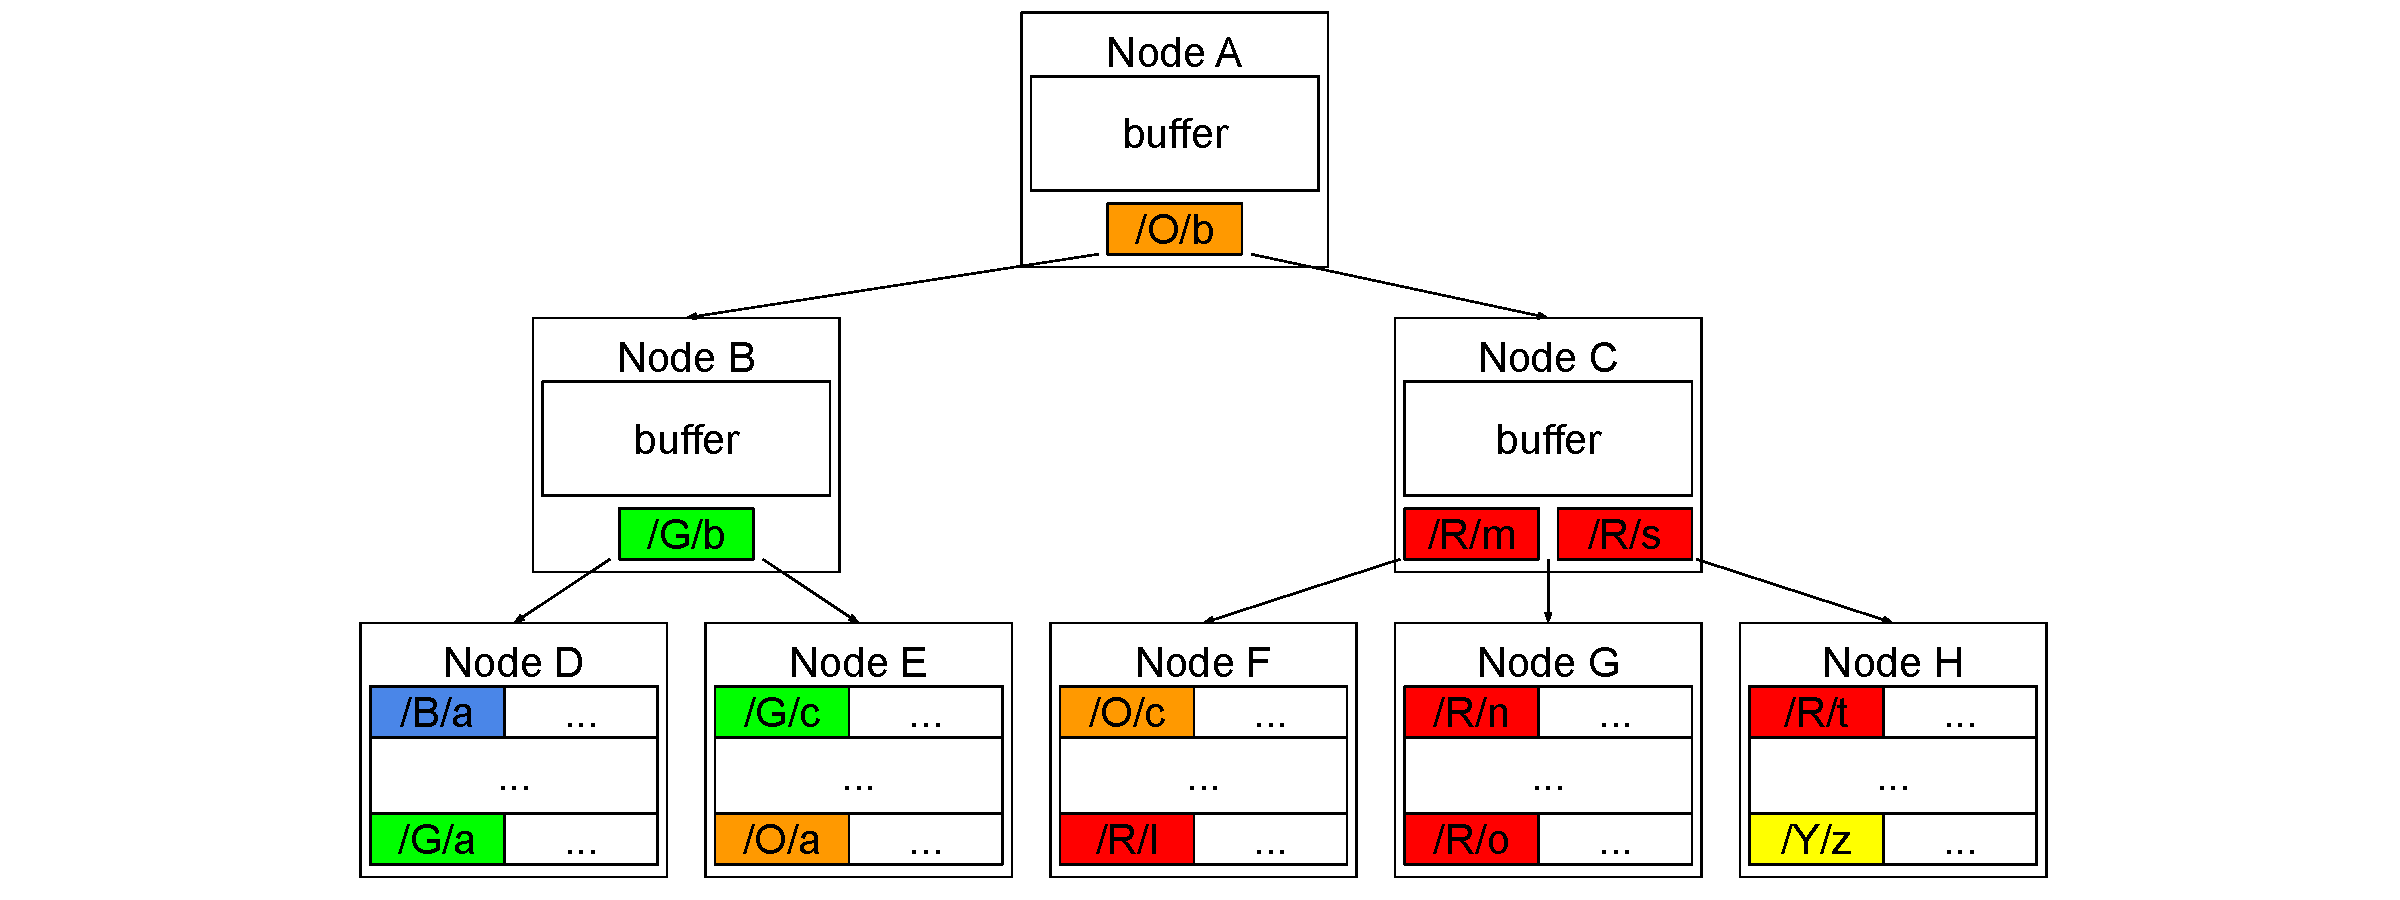
\includegraphics[width=.9\linewidth]{fig/slice-1}
        \caption{\label{subfig:slice-1} The \bet before tree surgery.}
    \end{subfigure}
    \begin{subfigure}{\textwidth}
        \centering
        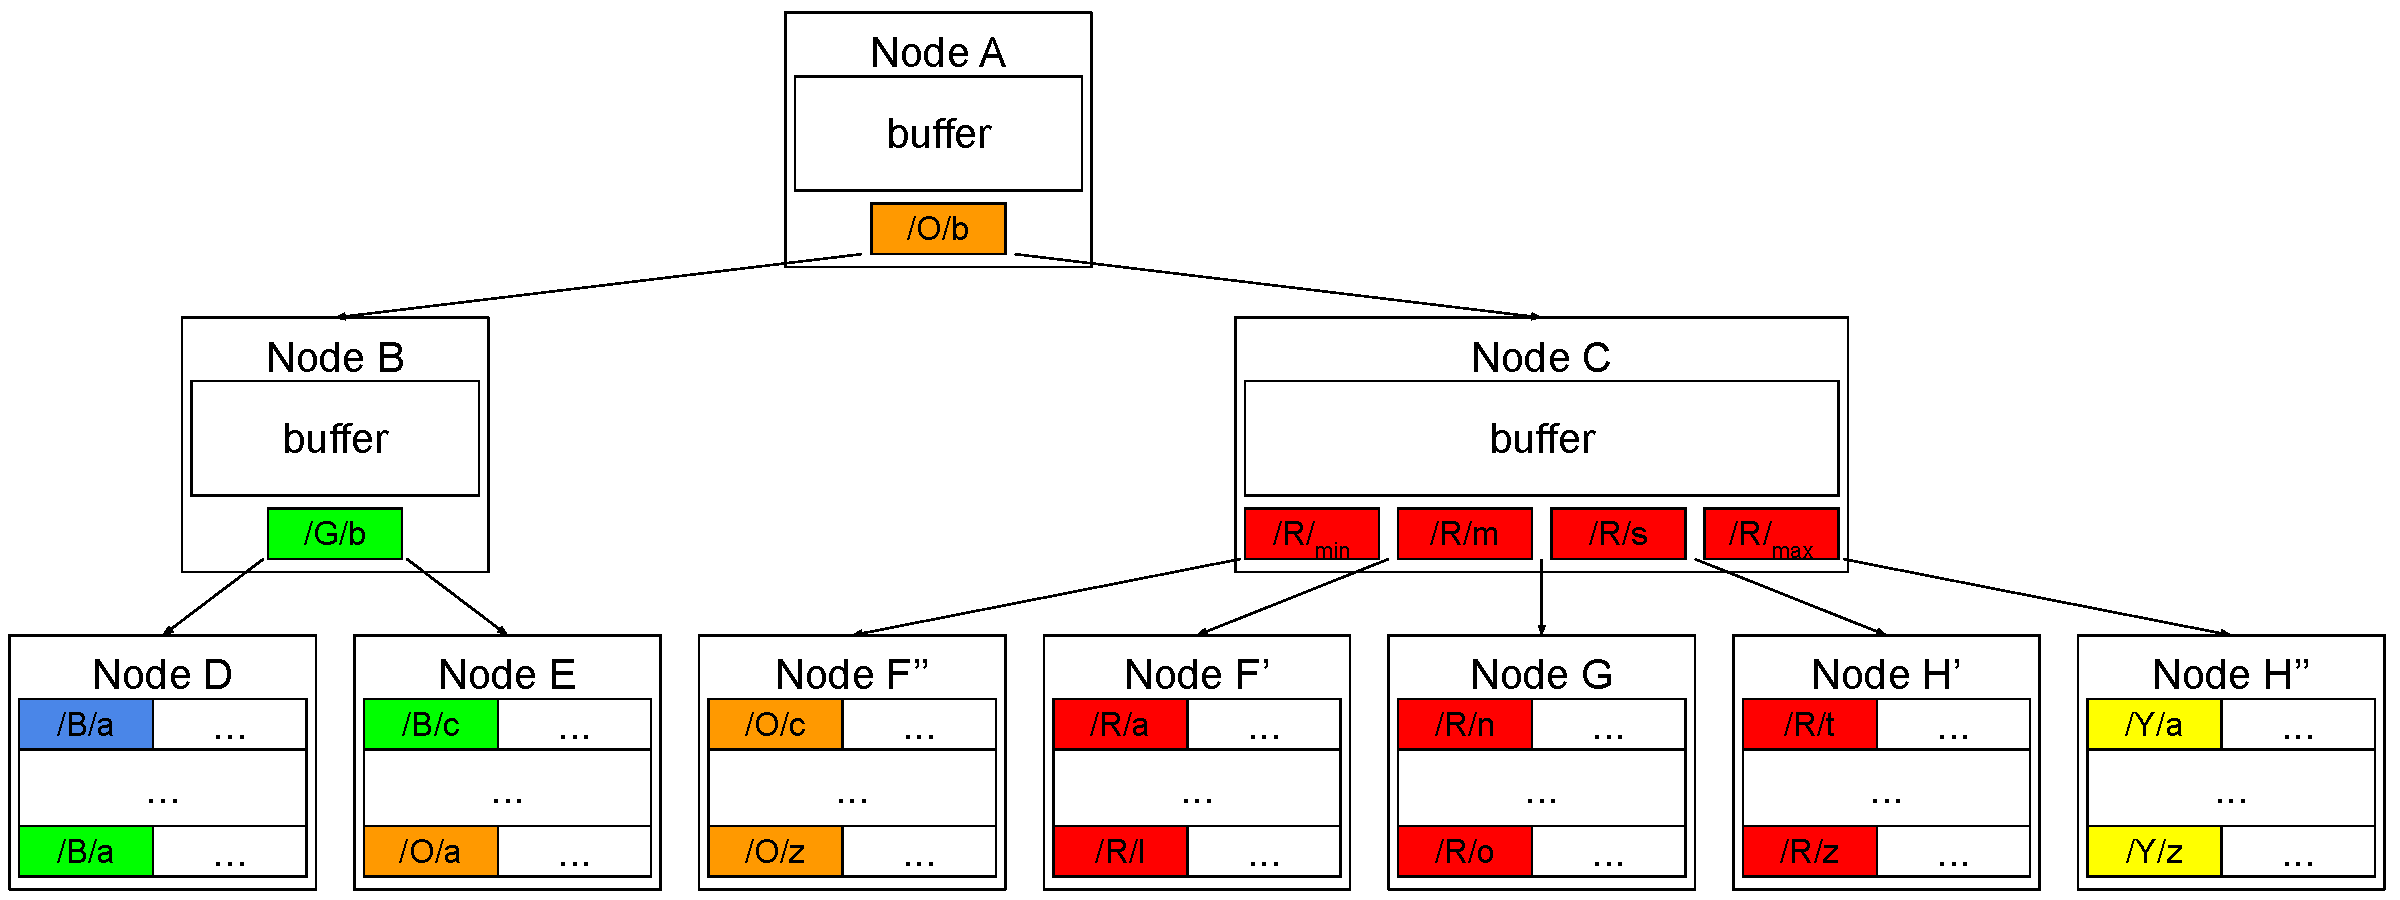
\includegraphics[width=.9\linewidth]{fig/slice-2}
        \caption{\label{subfig:slice-2} Tree surgery splits leaf nodes.}
    \end{subfigure}
    \begin{subfigure}{\textwidth}
        \centering
        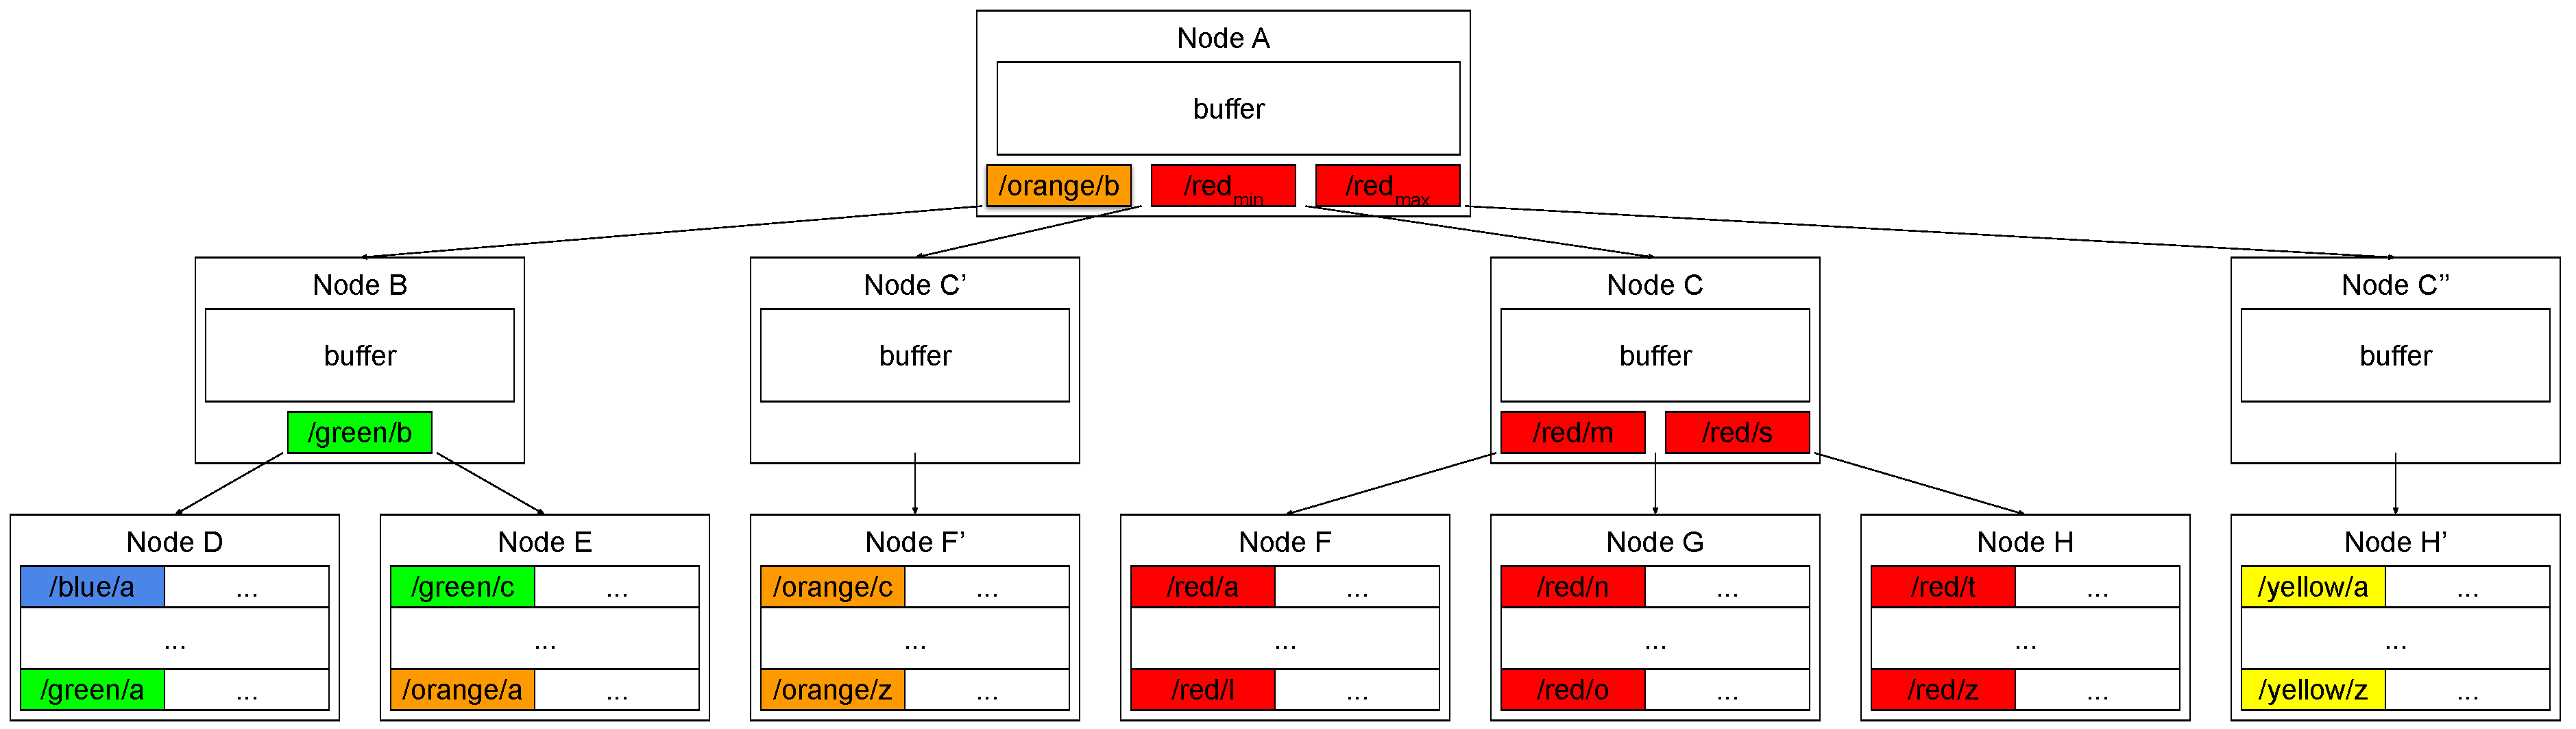
\includegraphics[width=.9\linewidth]{fig/slice-3}
        \caption{\label{subfig:slice-3} Tree surgery splits the LCA.}
    \end{subfigure}
    \caption[Tree surgery example]{\label{fig:slice}
        Tree surgery slices out an isolated subtree of prefix ``/red''.}
\end{figure}

The goal of tree surgery is to create an isolated subtree of a certain
prefix $p$ on the \bet.
In the \bet, each node covers a certain key range, bounded by the key range of
its parent and pivots in the parent.
For a certain key range $(p_{min}, p_{max})$ ($p_{min}$ and $p_{max}$ are the
minimum and maximum keys with prefix $p$, respectively), there are three types
of nodes: nodes whose range are completely out of the key range, nodes whose
range are completely in the key range, and nodes whose range partly overlapped
with the key range (called fringe nodes).

In renaming a file, the goal is to capture a range of contiguous keys and
logically move these key/value pairs to a different point in the tree.
For anything large enough to warrant using this rename approach,
some \bet nodes will exclusively store messages or key/value pairs
for the source or destination.
Some nodes may also include unrelated messages or key/value pairs
before and after this key range in sort order;
within the \bet these nodes will be along the left and right side of the nodes
that store only the messages or key/value pairs of interest.

An important abstraction for tree surgery is the \textbf{LCA}
(Lowest Common Ancestor) of two keys: the LCA is the \bet node lowest in the
tree on the search path for both keys (and hence including all keys in between).
During a range rename, the source and destination key ranges will each have an
LCA, and their LCAs may be the same node.

The first step in tree surgery is to find the source LCA and destination LCA.
In the process of identifying the LCAs, we also flush any pending messages for
the source or destination key range, so that they are buffered at or below the
corresponding LCAs.

\paragraph{Slicing}  The second step is to slice out the source and destination
key ranges from any shared nodes.
The goal of slicing is to separate unrelated key-value pairs that are not being
moved but are packed into the same \bet node as the key ranges to be move.
Slicing uses the same  code used for standard \bet node splits, but slicing
divides the node at the slicing key rather than picking a key in the middle of
the node.
As a result, slicing may result in nodes that temporarily violate constraints on
target node size and fanout.
However, these are performance, not correctness, constraints, so we can let
queries continue concurrently, and we restore these invariants before completing
the rename.

Our implementation requires that the source and destination LCA be at the same
height for the next step.
Thus, if the LCAs are not at the same level of the tree, we slice up to an
ancestor of the higher LCA.
The goal of this choice is to maintain the invariant that all \bet leaves be
at the same depth.

After this swap completes, and the locks are released,
new searches or updates for the destination will descend into the new subtree.

\paragraph{Healing}  Our \bet implementation maintains the
invariant that all internal nodes have between 4 and 16 children,
which bounds the height of the tree.  After the transplant completes,
however, there may be a number of in-memory \bet nodes at the fringe
around the source and destination that have fewer than 4 children.

We handle this situation by triggering a rebalancing within the tree.
Specifically, if a node has only one child, the slicing process will merge
it after completing the work of the rename.
After the transplant completes, there may be a number
of \bet nodes in memory at the fringe around the
source and destination that have fewer children than desired.
The healing process merges these smaller nodes back together,
using the same approach as a typical \bet merge.  At this point, it is also
possible that this could trigger a rebalancing within the tree.

One very important optimization we found as part of healing was to
agressively merge {\em stalks}, or new descendants of an LCA with
only a single child.
When the source and destination LCA are at different height, slicing
will creates some nodes with a single child.
Traversing these stalks undermines the logarithmic search time one would
expect from a tree, and created significant performance overheads.
After healing, we immediately merge nodes at the fringe
to a normal fanout in \bet.

\paragraph{Crash Consistency} \betrfs relies on three on-disk data structures to
ensure crash consistency: the trees, a block table indicating the disk blocks
used by the trees, and a write-ahead redo log. In general, \betrfs ensures crash
consistency by appending pending messages to the redo log and then applying
messages to the tree in a copy-on-write manner.
At periodic intervals (by default every 60 seconds), \betrfs ensures that there
is a consistent, sharp checkpoint of the tree on disk.
After a crash, \betrfs reads the last checkpointed tree and replays the redo log
after the checkpoint.
Range rename works within this framework.

A range rename is {\em logically applied} to the tree as soon as
(1) the range-rename message is added to the redo log and
(2) tree surgery locks the root of the tree.
The range rename is durable as soon as the redo log entry is written to disk.
If the system crashes after a range rename is logged, the recovery will see a
prefix of the message history that includes the range-rename message, and the
tree surgery will be redone in response to the range-rename message.
After both the tree surgery and the subsequent checkpoint of the tree complete,
there is no need to repeat the tree surgery after a crash.

We note that the current implementation does tree surgery immediately after the
message is placed in the redo log.
It is possible to batch range rename messages and apply them lazily,
but we leave this for future work.
As a result of this choice, however, there are fewer cases to reason about
in understanding crash consistency.

Tree surgery walks down the tree and locks the nodes along the path
hand-over-hand until either the source LCA or the destination LCA is reached.
Then, until tree surgery completes, all fringe nodes, the LCAs, and the parents
of LCAs are locked in memory and dirtied.
Upon tree surgery completion, these nodes will be unlocked.
Because the checkpoint process must grab the locks of all involved node before
writing them to disk,
no intermediate state of slicing will be exposed to a checkpoint.
Dirty nodes may be written back to disk, copy-on-write, before checkpointing
under memory pressure.
However, because the recovery process always starts from the last checkpoint and
the last block table in which these newly allocated nodes is not reachable,
these nodes with uncheckpointed state will be marked as free during crash
recovery.

If the system crashes after tree surgery begins but before surgery completes,
the recovery code will see a consistent checkpoint of the tree as it was
before the tree surgery.
The same is true if the system crashes after tree surgery but before dirty nodes
are written back to disk.
Because a checkpoint flushes all dirty nodes, if the system crashes after a
checkpoint, all nodes affected by tree surgery will be on disk.
We checked this functionality with crash recovery unit tests.
We ran the system in QEMU and crashed the system both before a rename completed
and before the rename log had been flushed;
we ensured that \betrfs restored the tree to the state before the tree surgery.

Tree surgery maintains the transactional properties of \betrfs.
It is performed at the commit stage of a range-rename transaction,
and thus aborting a range-rename transaction leaves no trace on the tree.
In the case of a crash, the tree surgery, which is encoded as a range-rename
message in the redo log, will be redone when the recovery process replays the
redo log.
The key to maintaining failure-atomicity of surgery is that all the involved
nodes must be locked in memory in the same batch to ensure the checkpoint has
a consistent snapshot of the tree at a point in time before or after,
but not during, the tree surgery.

At the file system level, \betrfs has similar crash consistency semantics to
metadata-only journaling in ext4.
The \bet implementation itself implements full data journaling, but \betrfs
allows file writes to be buffered in the VFS, weakening this guarantee
end-to-end.
Specifically, file writes may be buffered in the VFS caches, and are only logged
in the recovery journal once the VFS writes back a dirty page (e.g., upon an
{\tt fsync} or after a configurable period).
Changes to the directory tree structure, such as a {\tt rename} or {\tt mkdir}
are persisted to the log immediately.
Thus, in the common pattern of writing to a temporary file and then renaming it,
it is possible for the rename to appear in the log before the writes.
In this situation and in the absence of a crash, the writes will eventually be
logged with the correct, renamed key, as the in-memory inode will be up-to-date
with the correct \bet key.
If the system crashes, these writes can be lost; as with a metadata-journaled
file system, the developer must issue an {\tt fsync} before the {\tt rename} to
ensure the data is on disk.

\paragraph{Latency} A rename returns to the user once a log entry is in the
journal and the root node of the \bet is locked.
At this point, the rename has been applied in the VFS to in-memory metadata,
and as soon as the log is fsynced, the rename is durable.

We then hand off the rest of the rename work to two background threads
to do the cutting and healing.
The prototype in this paper only allows a backlog of one pending, large rename,
since we believe that concurrent renames are relatively infrequent.
The challenge in adding a rename work queue is ensuring consistency between the
work queue and the state of the tree.

\paragraph{Atomicity and Transactions}
The \bet in \betrfs implements multi-version concurrency control by augmenting
messages with a logical timestamp.
Messages updating a given key range are always applied in logical order.
Multiple messages can share a timestamp, giving them transactional semantics.

To ensure atomicity for a range rename, we create an MVCC ``hazard'':
read transactions ``before'' the rename must complete before the surgery
can proceed.
Tree nodes in \betrfs  are locked with reader-writer locks.
We write-lock tree nodes hand-over-hand, and left-to-right to identify
the LCAs.  Once the LCAs are locked, this serializes any new read or write
transactions until the rename completes.  The lock at the LCA creates
a ``barrier''---operations can complete ``above'' or ``below'' this lock
in the tree, although the slicing will wait for concurrent
transactions to complete before write-locking that node. Once the transplant
completes, the write-locks on the parents above LCAs are released.

In practice, \betrfs has a reader-writer lock in each in-memory inode to prevent
concurrent transactions from happening during a rename,
but this would be a concern in applying this technique to a general-purpose
key-value store or database that uses MVCC.

For simplicity, before the range rename is applied, we ensure that all messages
representing changes in the affected key range(s) that logically occurred before
the range rename are flushed below the LCA.
All messages that logically occur after the rename follow the new path through
the tree to the destination or source.
This strategy ensures that, when each message is flushed and applied, it sees a
point-in-time consistent view of the subtree.

\paragraph{Complexity} In the worst case, at most 4 slices are performed.
Slices go from the parent of the LCA to the leaf,
and nodes along this path are dirtied.
If the root of the tree is the LCA, a new root is inserted above the current
root for slicing.
These nodes will need to be read, if not in cache,
and written back to disk as part of the checkpointing process.
Therefore the number of IOs is at most proportional to the height of the \bet,
which is logarithmic in the size of the tree.

Let $N$ be the number of entries in a \bet, i.e., the number of files plus
directories in the metadata tree and the number of data blocks in the data tree.
Let $B$ be the size of a node.
And let $\varepsilon\in(0,1]$ be a design-time tuning parameter that adjusts the
fanout.
In the worst case, $O(\frac{\log_B{N}}{\varepsilon})$ (tree height)
I/Os will be performed  during a rename as a result of this design.

\subsection{Key lifting}

After tree surgery completes, there will be a subtree where the keys
are not coherent with the new location in the tree.  As part of a
rename, the prefixes of all keys in this subtree need to be updated.
For example, suppose we execute \texttt{`mv /foo /bar'}.  After surgery,
any messages and
key/value pairs for file \texttt{/foo/file} will still have a key that
starts with \texttt{/foo}.  These keys need to be changed to begin
with \texttt{/bar}.  The particularly concerning case is when {\tt
  /foo} is a very large subtree and has interior nodes that would
otherwise be untouched by the tree surgery step; our goal is to leave
these nodes untouched as part of rename, and thus reduce the cost of
key changes from the size of the rename tree to the height of the
rename tree.

We note that full-path keys in our tree are highly redundant.
Our solution
reduces the work of changing keys by reducing the redundancy of how
keys are encoded in the tree.
Consider the prefix encoding for a sequence
of strings.  In this compression method, if two strings share a
substantial longest common prefix (lcp), then that lcp is only stored
once.  We apply this idea to \bets. % by changing the way that nodes store keys.
The lcp of all keys in a subtree is removed from the keys and stored in the
subtree's parent node.
We call this approach \textbf{key lifting} or
simply \textbf{lifting} for short.

At a high level, each parent in a lifted \bet stores
each child's common, lifted key prefix alongside the pointer to the child.
Child nodes only store differing key suffixes.
This approach encodes the complete key in the path taken to reach a given node.

This solution leaves nodes interior to the subtree to be unmodified as part of a range rename.
Specifically, part of finding an LCA during tree surgery ensures that the prefix to be renamed
is lifted into the parent.

One can then modify the prefix for a lifted subtree by only modifying the
parent node.
This solution
eliminates the need to change key and pivot prefixes in all nodes of a subtree.

Lifting requires a schema-level invariant that keys with a common prefix are adjacent
in the sort order.  As a simple example, if one uses {\tt memcmp} to compare keys (as \betrfs does),
then lifting will be correct.  This invariant ensures that, if there is a common prefix between any two pivot keys,
all keys in that child will have the same prefix, which can be safely lifted.
More formally:
\begin{invariant}
Let $T'$ be a subtree in a \bet with full-path indexing.  Let $p$ and
$q$ be the pivots that enclose $T'$.  That is, if $T'$ is not the first
or last child of its parent, then $p$ and $q$ are the enclosing pivots
in the parent of $T'$.  If $T'$ is the first child of its parent, then
$q$ is the first pivot and $p$ is the left enclosing pivot of the parent of $T'$.

Let $s$ be the longest common prefix of $p$ and $q$.  Then all keys
in $T'$ begin with $s$.
\end{invariant}

\textbf{Figures Here}

Reads can reconstruct the full key by concatenating prefixes during a
root-to-leaf traversal.  In principle, one need not store the lifted prefix ($s$)
in the tree, as it can be computed from the pivot keys.
In our implementation, we do memorize the lifted prefix for efficiency.

As messages are flushed to a child, they
are modified to remove the common prefix.
Similarly, node splits and merges ensure that
any common prefix between the pivot keys is lifted out.
It is possible for all of the keys in $T'$ to
share a common prefix that is longer than $s$,  but we only lift
$s$ because maintaining this amount of lifting hits a sweet spot: \textit{it
is enough to guarantee fast key updates during renames, but it
requires only local information at a parent and child  
during splits, merges, and insertions.}

Lifting  is completely transparent to the file system.
From the file system's perspective, it is still indexing data with a
key/value store that is keyed by full-path; the only difference from the file
system's perspective is that the key/value store completes some
operations faster.

\paragraph{Lifting and Renames}
In the case of renames, lifting dramatically reduces the work to update
keys.  During a rename from $a$ to $b$, we slice out a sub-tree
containing exactly those keys that have $a$ as a prefix.  By the
lifting invariant, the prefix $a$ will be lifted out of the sub-tree,
and the parent of the sub-tree will bound it between two pivots whose
common prefix is $a$ (or at least includes $a$---the pivots may have
an even longer common prefix).  After we perform the pointer swing,
the sub-tree will be bounded in its new parent by pivots that have $b$
as a common prefix.  Thus, by the lifting invariant, all future queries
will interpret all the keys in the sub-tree has having $b$ as a prefix.
Thus, with lifting, the pointer swing implicitly performs the batch key-prefix
replacement, completing the rename.

\paragraph{Complexity} During tree surgery, there is lifting work
along all nodes that are sliced or merged.  However, the number of
such nodes is at most proportional to the height of the tree.
Thus, the number of nodes that must be lifted after a rename is no more than
the nodes that must be sliced during tree surgery, and proportional to the height
of the tree.

After slicing out the subtree containing all the source keys involved in the rename,
the two source slicing keys become the two pivots bounding the source subtree in the
parent.
Because the common prefix of the two source slicing keys is the old prefix,
the old prefix is lifted from the source subtree.
Then, by inserting the subtree
to the new location that is bounded by two destination slicing keys with the new prefix,
all the keys in the subtree are updated immediately.
An end-to-end example of renaming is illustrated in Figure~\ref{fig:e2e}.
In this example, each slicing step lifts the old-prefix /red. By the time the slice reaches the LCA,
the old-prefix /red is lifted out of the entire subtree.

\subsection{Put them together}

\textbf{Figures Here}

\section{Summary}

